\documentclass[tikz,border=2pt]{standalone}
\usepackage{amsmath}
\usepackage{pgfplots}
\pgfplotsset{compat=1.18}

\begin{document}
% A jump at x0: the value f(x0) sits on the right branch, so f is right-continuous at x0 but not
% left-continuous (the left branch approaches a different value).
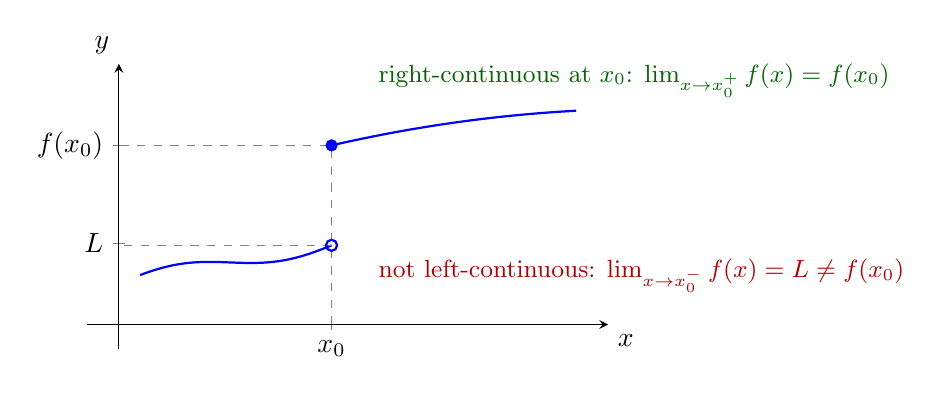
\begin{tikzpicture}
	\begin{axis}[
		axis lines=middle,
		xmin=-0.3, xmax=4.6,
		ymin=-0.3, ymax=3.2,
		xtick={2}, xticklabels={$x_0$},
		ytick={1,2.2}, yticklabels={$L$,$f(x_0)$},
		xlabel={$x$}, ylabel={$y$},
		xlabel style={below right}, ylabel style={above left},
		samples=100, smooth, clip=false,
		width=8.2cm, height=5.2cm
		]
		\addplot[thick, blue, domain=0.2:2] {0.5+0.25*x+0.1*sin(deg(3*x))};
		\addplot[thick, blue, domain=2:4.3] {2.2+0.3*(x-2)-0.05*(x-2)^2};
		\addplot[only marks, mark=o, mark size=2pt, blue, thick, fill=white] coordinates {(2,{0.5+0.5+0.1*sin(deg(6))})};
		\addplot[only marks, mark=*, blue] coordinates {(2,2.2)};
		\draw[dashed, gray] (axis cs:2,0) -- (axis cs:2,2.2) -- (axis cs:0,2.2);
		\draw[dashed, gray] (axis cs:2,{0.5+0.5+0.1*sin(deg(6))}) -- (axis cs:0,{0.5+0.5+0.1*sin(deg(6))});
		\node[green!40!black, anchor=west, font=\small, align=left] at (axis cs:2.35,3.0) {right-continuous at $x_0$: $\lim_{x\to x_0^+}f(x)=f(x_0)$};
		\node[red!70!black, anchor=west, font=\small, align=left] at (axis cs:2.35,0.6) {not left-continuous: $\lim_{x\to x_0^-}f(x)=L\neq f(x_0)$};
	\end{axis}
\end{tikzpicture}
\end{document}
